\documentclass[12pt, a4paper, reqno, oneside]{book}
\usepackage[left=2.5cm, right=2cm, top=2cm, bottom=2cm]{geometry}
\usepackage{amsmath,amssymb,amsfonts,amsthm}
\usepackage{microtype}
\usepackage{indentfirst}
\usepackage{fontspec}
\setmainfont{Times New Roman}
\usepackage[vietnamese]{babel}
\usepackage{graphicx}
\usepackage{float}
\usepackage{listings}
\usepackage[dvipsnames]{xcolor}
\usepackage{tikz}
\usetikzlibrary{calc}
\usepackage{array}
\usepackage{titlesec}
\usepackage{fancyhdr}
\usepackage{tabularx}
\usepackage[square,numbers]{natbib}
\usepackage[labelfont=bf, textfont=it, justification=centering]{caption}
\usepackage{booktabs}
\fancyhf{}
\fancyhead[L]{\small{\leftmark}}
\fancyfoot[C]{ \thepage}
\setlength{\headheight}{16pt}
\captionsetup{labelfont={color=blue, bf}, textfont={color=black, it}}

\usepackage[colorlinks,bookmarksopen,bookmarksnumbered,citecolor=blue, colorlinks=true,linkcolor=blue,urlcolor=blue]{hyperref}

\renewcommand{\baselinestretch}{1.25}

\newcommand \chap[1]{%
  \chapter*{#1}%
  \phantomsection%
  \addcontentsline{toc}{chapter}{#1}
  \markboth{#1}{}
}
\newcommand \sect[1]{%
  \section*{#1}%
  \phantomsection%
  \addcontentsline{toc}{section}{#1}}

\renewcommand{\theequation}{\arabic{chapter}.\arabic{equation}}
\newtheorem{lemma}{\bf Bổ đề}[chapter]
\newtheorem{theorem}{\bf Định lý}[chapter]
\newtheorem{proposition}{\bf Mệnh đề}[chapter]
\newtheorem{corollary}{\bf Hệ quả}[chapter]
\newtheorem{definition}{\bf Định nghĩa}[chapter]
\newtheorem{remark}{\bf Chú ý}[section]

% Mức tiêu đề subsubsubsection
\titleclass{\subsubsubsection}{straight}[\subsection]
\newcounter{subsubsubsection}[subsubsection]
\renewcommand\thesubsubsubsection{\thesubsubsection.\arabic{subsubsubsection}}
\renewcommand\theparagraph{\thesubsubsubsection.\arabic{paragraph}}

\titleformat{\subsubsubsection}
  {\normalfont\normalsize\bfseries}{\thesubsubsubsection}{1em}{}
\titlespacing*{\subsubsubsection}
{0pt}{3.25ex plus 1ex minus .2ex}{1.5ex plus .2ex}

\makeatletter
\renewcommand\paragraph{\@startsection{paragraph}{5}{\z@}%
  {3.25ex \@plus1ex \@minus.2ex}%
  {-1em}%
  {\normalfont\normalsize\bfseries}}
\renewcommand\subparagraph{\@startsection{subparagraph}{6}{\parindent}%
  {3.25ex \@plus1ex \@minus .2ex}%
  {-1em}%
  {\normalfont\normalsize\bfseries}}
\def\toclevel@subsubsubsection{4}
\def\toclevel@paragraph{5}
\def\toclevel@paragraph{6}
\def\l@subsubsubsection{\@dottedtocline{4}{7em}{4em}}
\def\l@paragraph{\@dottedtocline{5}{10em}{5em}}
\def\l@subparagraph{\@dottedtocline{6}{14em}{6em}}
\makeatother

\setcounter{secnumdepth}{4}
\setcounter{tocdepth}{4}

% Thư mục hình
\graphicspath{{./figs/}}

\definecolor{mygreen}{rgb}{0,0.6,0}
\definecolor{mygray}{rgb}{0.5,0.5,0.5}
\definecolor{mymauve}{rgb}{0.58,0,0.82}

\lstdefinestyle{customc}{
  belowcaptionskip=1\baselineskip,
  breaklines=true,
  frame=single,
  xleftmargin=\parindent,
  language=C,
  showstringspaces=false,
  basicstyle=\footnotesize\ttfamily,
  keywordstyle=\bfseries\color{green!40!black},
  commentstyle=\itshape\color{purple!40!black},
  identifierstyle=\color{blue},
  stringstyle=\color{orange},
  numbers=left,
  numberstyle=\tiny\color{gray},
  stepnumber=1, 
}
\lstset{escapechar=@,style=customc}

\newcolumntype{C}[1]{>{\centering\arraybackslash}p{#1}}

\begin{document}
\selectlanguage{vietnamese}
\hypersetup{pageanchor=false}

% ==================== TRANG BÌA NGOÀI ====================
\begin{titlepage}
\begin{center}
	\begin{tikzpicture}[overlay,remember picture]
	    \draw [line width=3pt,rounded corners=0pt]
	        ($ (current page.north west) + (20mm,-20mm) $)
	        rectangle
	        ($ (current page.south east) + (-15mm,20mm) $);
	    \draw [line width=1pt,rounded corners=0pt]
	        ($ (current page.north west) + (21.5mm,-21.5mm) $)
	        rectangle
	        ($ (current page.south east) + (-16.5mm,21.5mm) $);
	\end{tikzpicture}
	\\[1mm]
    \centerline{\bf ĐẠI HỌC QUỐC GIA HÀ NỘI}
    \centerline{\bf TRƯỜNG ĐẠI HỌC CÔNG NGHỆ}
    
    \vspace*{1.5cm}
    \large
        \begin{figure}[H]
        \centering
        
\includegraphics[width=0.23\linewidth]{figs/uet.jpg}
        \end{figure}
    \vspace*{0.8cm}
    \centerline{\bf VŨ TIẾN TUẤN TRUNG}
    \vspace*{2.0cm}
    \centerline{\Large\bf HỌC BIỂU DIỄN ĐỘC LẬP ĐẶC THÙ XE}
    \centerline{\Large\bf CHO HỆ THỐNG PHÁT HIỆN XÂM NHẬP}
    \centerline{\Large\bf MẠNG CAN BUS ĐA PHƯƠNG TIỆN}
    \vspace*{2.2cm}
    \centerline{\bf KHÓA LUẬN TỐT NGHIỆP ĐẠI HỌC}
    \vspace*{0.2cm}
    \centerline{\bf Ngành: Hệ thống Thông tin}
    
    \vfill
    \centerline{\bf Hà Nội - 2026}
    \vspace{13pt}
\end{center}
\end{titlepage}

\newpage

% ==================== TRANG BÌA TRONG ====================
\begin{titlepage}
\begin{center}
	\begin{tikzpicture}[overlay,remember picture]
	    \draw [line width=3pt,rounded corners=0pt]
	        ($ (current page.north west) + (20mm,-20mm) $)
	        rectangle
	        ($ (current page.south east) + (-15mm,20mm) $);
	    \draw [line width=1pt,rounded corners=0pt]
	        ($ (current page.north west) + (21.5mm,-21.5mm) $)
	        rectangle
	        ($ (current page.south east) + (-16.5mm,21.5mm) $);
	\end{tikzpicture}
	\\[1mm]
    \centerline{\bf ĐẠI HỌC QUỐC GIA HÀ NỘI}
    \centerline{\bf TRƯỜNG ĐẠI HỌC CÔNG NGHỆ}
    \vspace*{1.5cm}
    \large
        \begin{figure}[H]
        \centering
        
\includegraphics[width=0.23\linewidth]{figs/uet.jpg}
        \end{figure}
    \vspace*{0.8cm}
    \large
    \centerline{\bf VŨ TIẾN TUẤN TRUNG}
    \vspace*{1.8cm}
    \centerline{\Large\bf HỌC BIỂU DIỄN ĐỘC LẬP ĐẶC THÙ XE}
    \centerline{\Large\bf CHO HỆ THỐNG PHÁT HIỆN XÂM NHẬP}
    \centerline{\Large\bf MẠNG CAN BUS ĐA PHƯƠNG TIỆN}
    \vspace*{1.6cm}
    \centerline{\bf KHÓA LUẬN TỐT NGHIỆP ĐẠI HỌC}
    \vspace*{0.2cm}
    \centerline{\bf Ngành: Hệ thống Thông tin}
    
    \vspace*{1.4cm}
    \centerline{\bf Cán bộ hướng dẫn:}
    \centerline{\bf PGS. TS. Nguyễn Ngọc Hóa}
    
    \vfill
    \centerline{\bf Hà Nội - 2026}
    \vspace{13pt}
\end{center}
\end{titlepage}

\newpage
\pagenumbering{gobble}

% ==================== LỜI CẢM ƠN ====================
\chapter*{Lời cảm ơn}
\vspace{20pt}

Em xin bày tỏ lòng biết ơn sâu sắc và chân thành nhất tới Thầy giáo hướng dẫn, PGS. TS. Nguyễn Ngọc Hóa, người đã luôn tận tình định hướng, hỗ trợ và động viên em trong suốt quá trình thực hiện nghiên cứu này. Những kiến thức sâu rộng, những phản biện học thuật sắc sảo cùng sự chỉ bảo tận tâm của Thầy là yếu tố quyết định giúp em vượt qua các thách thức kỹ thuật phức tạp và hoàn thành khóa luận tốt nghiệp này.

Các công cụ trí tuệ nhân tạo (AI-assisted tools) đã được sử dụng hỗ trợ tổ chức cấu trúc văn bản, rà soát ngữ pháp và tối ưu hóa mã nguồn thực nghiệm. Tác giả chịu trách nhiệm hoàn toàn đối với thiết kế nghiên cứu, thiết lập thực nghiệm, thu thập dữ liệu, mã nguồn và toàn bộ các kết luận khoa học được trình bày trong khóa luận này.

Mặc dù đã nỗ lực cao nhất để đảm bảo tính chặt chẽ và chuẩn xác học thuật, tác giả nhận thức rằng nghiên cứu vẫn còn những điểm có thể tiếp tục hoàn thiện. Em xin chân thành cảm ơn và trân trọng đón nhận mọi ý kiến đóng góp quý báu từ Hội đồng chấm khóa luận để nâng cao hơn nữa chất lượng của công trình nghiên cứu này.

Xin chân thành cảm ơn!

\newpage

% ==================== LỜI CAM ĐOAN ====================
\chapter*{Lời cam đoan}
\vspace{20pt}

Tôi xin cam đoan khóa luận tốt nghiệp này là công trình nghiên cứu khoa học độc lập của bản thân, được thực hiện dưới sự hướng dẫn trực tiếp và tận tình của PGS. TS. Nguyễn Ngọc Hóa. Tôi khẳng định rằng tài liệu này chưa từng được nộp, dù là toàn bộ hay một phần, để nhận bất kỳ học vị hay chứng chỉ chuyên môn nào tại cơ sở đào tạo này hay bất kỳ cơ sở nào khác.

Mọi nguồn trích dẫn, tài liệu tham khảo và các công trình liên quan được sử dụng trong nghiên cứu này đều đã được thừa nhận và trích dẫn đầy đủ, minh bạch theo chuẩn mực học thuật quốc tế. Bên cạnh đó, tôi cam đoan rằng toàn bộ dữ liệu thực nghiệm và các kết quả phân tích thống kê được trình bày là kết quả chân thực thu được từ quá trình chạy thử nghiệm khách quan, độc lập và có khả năng tái lập.

Tôi hoàn toàn chịu trách nhiệm về tính trung thực của lời cam đoan này theo các quy định và chính sách về liêm chính học thuật của Trường Đại học Công nghệ, Đại học Quốc gia Hà Nội.

\begin{flushright}
{\it Tác giả khóa luận}
\hskip 1.5cm\quad

\vskip 2cm
{\bf Vũ Tiến Tuấn Trung }  \quad\ \quad
\end{flushright}
\newpage

% ==================== TÓM TẮT KHÓA LUẬN ====================
\chapter*{Tóm tắt khóa luận}
\vspace{20pt}

Các hệ thống phát hiện xâm nhập mạng Controller Area Network (CAN IDS) thường công bố hiệu năng phân loại rất cao trong điều kiện đánh giá ngẫu nhiên hoặc nội bộ trên cùng một dòng xe. Tuy nhiên, độ tin cậy của chúng thường sụp đổ nghiêm trọng khi triển khai trên một dòng xe chưa từng thấy (unseen vehicle) hoặc khi đối mặt với các hình thức tấn công mới. Khóa luận này nghiên cứu hiện tượng chuyển dịch phân phối (distribution shift) bằng cách sử dụng bộ dữ liệu đối chuẩn \texttt{can-train-and-test} và đánh giá liệu một biểu diễn cấu trúc độc lập định danh xe có thể giải quyết sự phụ thuộc vào mã CAN-ID cụ thể hay không.

Luồng dữ liệu CAN được phân chia thành các cửa sổ trượt không chồng lấn với kích thước cố định $W = 64$ khung tin và được đánh giá trong 4 điều kiện kiểm thử zero-shot: dòng xe quen và tấn công quen (Điều kiện A), xe lạ với tấn công quen (Điều kiện B), xe quen với tấn công mới (Điều kiện C), và chuyển dịch kép cả xe lạ lẫn tấn công mới (Điều kiện D). Biểu diễn đề xuất loại bỏ triệt để các bit CAN-ID tuyệt đối mang đặc thù riêng của từng hãng xe, tích hợp thông tin tải dữ liệu (payload), mã độ dài (DLC), độ biến thiên payload cục bộ cùng ID, khoảng cách thời gian giữa 2 gói liên tiếp, thời gian chu kỳ của cùng ID, cùng các thống kê tần suất và xác suất chuyển tiếp ID trong cửa sổ. Mô hình Transformer Encoder được so sánh trực diện với mô hình Transformer dùng đặc trưng thô (Raw Transformer) và mô hình phân loại Structural XGBoost.

Trong thử nghiệm trọng tâm trên Tập dữ liệu 1 (Set 1), mô hình Transformer Cấu trúc (Structural Transformer) đạt điểm F1 nhãn tấn công lần lượt là $0.9035$, $0.9703$, $0.7094$, và $0.2332$ qua 4 Điều kiện A--D; trong khi đó mô hình Raw Transformer sụp đổ về $0.7649$, $0.0002$, $0.0$, và $0.0$. Mức cải thiện vượt bậc nhất được ghi nhận ở kịch bản chuyển giao sang xe lạ (Điều kiện B, xe Chevrolet Silverado) với tỷ lệ phát hiện (Recall) đạt $94.26\%$ và độ chính xác (Precision) đạt $99.97\%$ với FAR chỉ $2.17 / 100,000$ cửa sổ. Ở kịch bản chuyển dịch kép (Điều kiện D), mô hình cải thiện rõ rệt so với sự bất lực của mô hình thô. Các thực nghiệm kiểm chứng ngoại suy trên 4 hãng xe ngoài (Opel Astra, Ford 2019, Hyundai Sonata, Renault Clio) khẳng định tỷ lệ báo động giả bằng $0.00\%$ trên hành trình lái xe bình thường. Những phát hiện này chứng minh biểu diễn cấu trúc là hướng đi đầy hứa hẹn để bẻ gãy sự phụ thuộc vào mã CAN-ID nội xe.

\vspace{1em}
\noindent \textit{\textbf{Từ khóa:} Mạng Controller Area Network (CAN), an toàn an ninh ô tô, phát hiện xâm nhập (IDS), chuyển dịch phân phối đa phương tiện, biểu diễn cấu trúc phi định danh xe, Transformer.}

\newpage
\tableofcontents

\newpage
\listoffigures

\newpage
\listoftables

\newpage
\chapter*{Danh mục từ viết tắt}
\vspace{20pt}

\begin{table}[H]
\centering
\begin{tabular}{|m{2.5cm}|m{11cm}|}
\hline
\textbf{Viết tắt} & \textbf{Tên tiếng Anh (Ý nghĩa tiếng Việt)} \\ \hline
AI & Artificial Intelligence (Trí tuệ nhân tạo) \\ \hline
CAN & Controller Area Network (Mạng vùng điều khiển) \\ \hline
CNN & Convolutional Neural Network (Mạng nơ-ron tích chập) \\ \hline
DBC & Database for CAN (Cơ sở dữ liệu cấu hình thông điệp CAN) \\ \hline
DLC & Data Length Code (Mã độ dài trường dữ liệu) \\ \hline
DoS & Denial of Service (Tấn công từ chối dịch vụ) \\ \hline
ECU & Electronic Control Unit (Bộ điều khiển điện tử trên ô tô) \\ \hline
FAR & False Alarm Rate (Tỷ lệ báo động giả trên 100,000 cửa sổ) \\ \hline
FPR & False Positive Rate (Tỷ lệ dương tính giả) \\ \hline
IDS & Intrusion Detection System (Hệ thống phát hiện xâm nhập) \\ \hline
IVN & In-Vehicle Network (Mạng truyền thông nội xe) \\ \hline
MHSA & Multi-Head Self-Attention (Cơ chế tự chú ý đa đầu) \\ \hline
ML & Machine Learning (Học máy) \\ \hline
OBD-II & On-Board Diagnostics II (Cổng chẩn đoán tích hợp trên xe) \\ \hline
PR-AUC & Area under the Precision-Recall Curve (Diện tích dưới đường cong PR) \\ \hline
TPR & True Positive Rate / Sensitivity (Tỷ lệ bắt trúng xâm nhập) \\ \hline
XGBoost & eXtreme Gradient Boosting (Thuật toán tăng cường độ dốc) \\ \hline
\end{tabular}
\end{table}

% ==================== CHƯƠNG 1 ====================
\chap{Chương 1: Mở đầu}
\label{chap:introduction}
\pagestyle{fancy}
\pagenumbering{arabic}

\sect{1.1. Tính cấp thiết của đề tài}

Các phương tiện giao thông thông minh hiện đại ngày càng phụ thuộc sâu sắc vào mạng truyền thông nội xe Controller Area Network (CAN bus) để trao đổi thông điệp điều khiển thời gian thực giữa hàng chục đến hàng trăm Bộ điều khiển điện tử (Electronic Control Units - ECUs)~\cite{verma2024road,bozdal2020evaluation}. Giao thức CAN ban đầu được thiết kế ưu tiên tối đa cho tính thời gian thực và độ tin cậy cơ học, do đó hoàn toàn thiếu vắng các cơ chế bảo mật cơ bản như mã hóa nội dung (encryption) và xác thực nguồn gốc thông điệp (authentication)~\cite{koscher2010experimental,lampe2023cantrainandtest,bozdal2020evaluation}. Lỗ hổng cấu trúc này cho phép kẻ tấn công khi xâm nhập được vào đường truyền vật lý hoặc thông qua cổng chẩn đoán On-Board Diagnostics (OBD-II) có thể dễ dàng chèn, giả mạo, phát lại các khung tin độc hại nhằm làm tê liệt hoặc chiếm quyền kiểm soát phương tiện~\cite{checkoway2011comprehensive,verma2024road}. 

Đặc biệt, công trình nghiên cứu thực nghiệm mang tính bước ngoặt của Miller và Valasek (2015)~\cite{miller2015remote} đã chứng minh việc chiếm quyền điều khiển từ xa một chiếc xe Jeep Cherokee đang lưu thông trên đường cao tốc thông qua mạng di động tế bào, can thiệp trực tiếp vào hệ thống phanh, vô-lăng và hộp số, buộc nhà sản xuất phải triệu hồi khẩn cấp $1.4$ triệu xe. Bên cạnh đó, Cho và Shin (2016)~\cite{cho2016fingerprinting} trên diễn đàn USENIX Security cũng khẳng định rằng bất kỳ ECU nào bị tổn thương đều có thể thực hiện tấn công mạo danh (impersonation) hoàn hảo trên bus truyền thông. Do đó, việc nghiên cứu các Hệ thống Phát hiện Xâm nhập (Intrusion Detection Systems - IDSs) dựa trên học máy và học sâu cho mạng CAN đã trở thành ưu tiên an ninh hàng đầu~\cite{ghadi2026learning,althunayyan2025survey,song2020dcnn}.

Tuy nhiên, một rào cản lớn đang hạn chế việc ứng dụng thực tế của CAN IDS là khả năng tổng quát hóa chuyển giao giữa các dòng xe khác nhau (cross-vehicle generalization). Tuyệt đại đa số các nghiên cứu hiện nay đều huấn luyện và đánh giá mô hình trên dữ liệu thu thập từ duy nhất một dòng xe hoặc trong các điều kiện dữ liệu đồng nhất~\cite{kidmose2025cansleuth,koltai2026canwetrust}. Trong điều kiện đóng đó, mô hình học máy dễ dàng đạt được độ chính xác gần như tuyệt đối bằng cách học vẹt (memorizing) các đặc trưng đặc thù của dòng xe tập huấn, chẳng hạn như dải mã định danh CAN-ID tuyệt đối, tần suất chu kỳ phát cố định hay định dạng dữ liệu payload tĩnh. Những đặc trưng này thực chất phản ánh "dấu vết của dòng xe" chứ không phản ánh bản chất quy luật của hành vi tấn công~\cite{koltai2026canwetrust,lampe2023cantrainandtest}.

Hậu quả là, một mô hình IDS đạt F1-score trên $99\%$ khi thử nghiệm trên xe quen (Intra-vehicle) sẽ lập tức sụp đổ hoàn toàn khi triển khai trên một dòng xe lạ (Unseen vehicle) chưa từng xuất hiện trong tập huấn luyện~\cite{koltai2026canwetrust,kidmose2025cansleuth}. Điều này đặt ra yêu cầu cấp thiết: làm thế nào để xây dựng một kiến trúc IDS có khả năng học biểu diễn độc lập đặc thù xe (vehicle-agnostic representation), bóc tách được các quy luật bất biến về cấu trúc tranh chấp bus và biến thiên payload để phát hiện xâm nhập thành công trên các dòng xe mới mà không cần huấn luyện lại từ đầu.

\sect{1.2. Thách thức và bài toán nghiên cứu}

Việc xây dựng một hệ thống CAN IDS có khả năng hoạt động trên dòng xe chưa từng thấy đối mặt với 4 thách thức cốt lõi:
\begin{enumerate}
    \item \textbf{Sự sai khác mã định danh theo nhà sản xuất (DBC Heterogeneity):} Mỗi hãng sản xuất ô tô sử dụng các file cơ sở dữ liệu riêng (Database for CAN - DBC) được bảo mật nghiêm ngặt để gán chức năng cho các mã CAN-ID~\cite{lampe2023cantrain,lampe2024curated}. Cùng một chức năng điều khiển tốc độ hay góc lái, xe Chevrolet sử dụng tập CAN-ID hoàn toàn khác biệt so với xe Ford hay Hyundai~\cite{lampe2024curated}. Các mô hình nạp mã CAN-ID thô sẽ bị lạc lối hoàn toàn khi chuyển sang dòng xe mới.
    \item \textbf{Ảo ảnh chỉ số đánh giá do mất cân bằng dữ liệu cực đoan (The F1 Score Illusion):} Dữ liệu mạng CAN nội xe có tỷ lệ mất cân bằng nghiêm trọng giữa lưu lượng bình thường và lưu lượng tấn công ($38:1$ đến $900:1$). Theo định lý Base-Rate Fallacy của Stefan Axelsson (2000)~\cite{axelsson2000base}, việc sử dụng các chỉ số như Accuracy hoặc Weighted F1 sẽ tạo ra "con số cao giả tạo" do lớp đa số bình thường kéo điểm lên, che giấu sự sụp đổ hoàn toàn của khả năng phát hiện xâm nhập trên lớp thiểu số.
    \item \textbf{Giả định thế giới đóng (Closed-World Assumption):} Như Robin Sommer và Vern Paxson (IEEE S\&P 2010)~\cite{sommer2010outside} đã cảnh báo, các hệ thống IDS áp dụng máy học thường thất bại ngoài đời thực vì được tối ưu trong một "thế giới đóng". Khi bước ra "thế giới mở" với các biến động về phong cách lái và kiến trúc ECU mới, tỷ lệ báo động giả tăng vọt làm tê liệt toàn bộ hệ thống phòng thủ.
    \item \textbf{Sự đan xen giữa chuyển dịch xe và chuyển dịch kiểu tấn công:} Khi mô hình bị suy giảm hiệu năng, rất khó phân định nguyên nhân bắt nguồn từ sự thay đổi của kiến trúc xe hay do sự xuất hiện của biến thể tấn công mới.
\end{enumerate}

\sect{1.3. Mục tiêu và nhiệm vụ nghiên cứu}

Mục tiêu tổng quát của khóa luận là: \textbf{Nghiên cứu nguyên nhân suy giảm hiệu năng của CAN IDS dưới tác động của chuyển dịch phân phối đa phương tiện và đề xuất khung phương pháp học biểu diễn cấu trúc 32 chiều độc lập CAN-ID kết hợp mạng Transformer Encoder nhằm nâng cao khả năng phát hiện xâm nhập zero-shot trên dòng xe chưa từng thấy.}

Để đạt được mục tiêu trên, khóa luận giải quyết 4 câu hỏi nghiên cứu cụ thể:
\begin{itemize}
    \item \textbf{RQ1:} Hiệu năng của CAN IDS suy giảm như thế nào khi chuyển đổi giữa dòng xe quen, dòng xe lạ và các kiểu tấn công mới trong điều kiện đánh giá zero-shot?
    \item \textbf{RQ2:} Mức độ đóng góp và tính dễ bị tổn thương của từng nhóm đặc trưng (CAN ID thô, Payload, Thời gian $\Delta t$) đối với khả năng tổng quát hóa đa xe là gì?
    \item \textbf{RQ3:} Liệu một biểu diễn cấu trúc 32 chiều phi định danh CAN-ID có thể duy trì được khả năng phát hiện đa dạng các loại tấn công trên xe lạ mà không làm bùng phát báo động giả hay không?
    \item \textbf{RQ4:} Khung phương pháp đề xuất có khả năng kiểm chứng ngoại suy bền vững trên các bộ dữ liệu độc lập của các hãng xe châu Âu và châu Á (Opel, Ford, Hyundai) hay không, và đâu là ranh giới thất bại của mô hình?
\end{itemize}

\sect{1.4. Đóng góp khoa học của khóa luận}

Khóa luận mang lại 4 đóng góp chính cả về mặt phương pháp luận lẫn thực nghiệm:
\begin{enumerate}
    \item \textbf{Hình thức hóa bài toán chuyển giao zero-shot đa xe:} Thiết lập quy trình đánh giá chuẩn tắc trên 4 điều kiện chuyển dịch A, B, C, D của bộ dữ liệu \texttt{can-train-and-test}, bóc tách tường minh sự suy giảm do đổi xe và suy giảm do đổi đòn tấn công.
    \item \textbf{Thiết kế Động cơ Trích xuất Cấu trúc 32 Chiều (32-D Invariant Engine):} Loại bỏ $100\%$ các bit mã định danh CAN-ID tuyệt đối, thay thế bằng các đặc trưng bất biến vật lý về động lực học nhịp, độ biến thiên payload vi phân và quan hệ chuyển tiếp cục bộ trong cửa sổ.
    \item \textbf{Vạch trần "Ảo ảnh F1" trong y văn và đối sánh trực diện:} Tái lập ma trận nhầm lẫn gốc từ phụ lục bài báo *Brooke Lampe \& Weizhi Meng (Computers \& Security 2024)*~\cite{lampe2024curated}, chứng minh các baseline công bố F1 $>0.95$ thực chất bắt trúng $0\% - 3.8\%$ tấn công, trong khi mô hình Structural Transformer đề xuất nâng Attack Recall lên $\mathbf{94.26\%}$, Attack F1 đạt $\mathbf{0.9703}$ với tỷ lệ báo động giả cực thấp ($\text{FAR} = 2.17 / 100,000$).
    \item \textbf{Kiểm chứng ngoại suy nghiêm ngặt trên 4 hãng xe quốc tế:} Kiểm chứng độ bền vững trên 4 bộ dữ liệu ngoài gồm Opel Astra, Ford 2019, Hyundai Sonata và Car-Hacking Lab, đạt FAR $0.00\%$ trên lưu lượng xe chạy bình thường với thông lượng xử lý vượt mức $40,000$ khung hình/giây.
\end{enumerate}

\sect{1.5. Bố cục của khóa luận}

Nội dung khóa luận được tổ chức thành 6 chương:
\begin{itemize}
    \item \textbf{Chương 1 (Mở đầu):} Trình bày tính cấp thiết, thách thức, mục tiêu, câu hỏi nghiên cứu và các đóng góp chính.
    \item \textbf{Chương 2 (Cơ sở lý thuyết):} Trình bày giao thức mạng CAN, phân loại tấn công, hiện tượng chuyển dịch phân phối và hình thức hóa toán học bài toán.
    \item \textbf{Chương 3 (Các nghiên cứu liên quan):} Tổng quan y văn về các phương pháp IDS truyền thống, chuyển giao tri thức, biểu diễn đồ thị và phân tích các chỉ số đánh giá.
    \item \textbf{Chương 4 (Khung phương pháp đề xuất):} Chi tiết hóa kiến trúc 32 đặc trưng cấu trúc, bộ mã hóa chuỗi Transformer Encoder và quy trình huấn luyện Focal Loss.
    \item \textbf{Chương 5 (Kết quả thực nghiệm và Phân tích):} Báo cáo kết quả 4 phase, đối sánh trực diện với bài báo gốc, kiểm chứng đa hãng xe và thảo luận ranh giới khoa học.
    \item \textbf{Chương 6 (Kết luận và Hướng phát triển):} Tóm lược các kết quả đạt được, chỉ rõ hạn chế và gợi mở các hướng nghiên cứu tiếp theo.
\end{itemize}

% ==================== CHƯƠNG 2 ====================
\chapter{Chương 2: Cơ sở lý thuyết và Phát biểu bài toán}
\label{chap:background}

Chương này trình bày các nguyên lý kỹ thuật của giao thức CAN bus, phân tích hiện tượng chuyển dịch phân phối khi triển khai IDS đa phương tiện, tổng quan 5 bộ dữ liệu đối chuẩn và định nghĩa hình thức bài toán phát hiện xâm nhập theo cửa sổ trượt.

\section{Mạng CAN Bus và An toàn An ninh Mạng Nội xe}
\label{subsec:can_intrusion_detection}

Mạng Controller Area Network (CAN) là chuẩn giao thức bus truyền thông nối tiếp dạng quảng bá (broadcast), được phát triển nhằm kết nối liên thông các Bộ điều khiển điện tử (ECU) trong xe hơi hiện đại~\cite{song2020invehicle,lee2017otids,bozdal2020evaluation}. Tất cả các ECU trên xe đều chia sẻ chung một cặp dây dẫn vật lý vi sai (CAN\_High và CAN\_Low). Khung dữ liệu CAN tiêu chuẩn (CAN 2.0A) bao gồm trường định danh trọng tài 11-bit (CAN ID), mã chỉ độ dài dữ liệu ($\text{DLC} \in \{0, \dots, 8\}$), và trường dữ liệu chứa tối đa 8 byte payload~\cite{lampe2024curated}. 

Điểm đặc thù của CAN là gói tin không chứa địa chỉ gửi hay nhận. Thay vào đó, mã CAN ID đại diện cho ý nghĩa thông điệp và quyết định quyền ưu tiên chiếm quyền đường truyền trong quá trình trọng tài bit (bitwise arbitration): khung tin nào có giá trị số CAN ID nhỏ hơn sẽ giành chiến thắng và được quyền phát trước~\cite{song2020invehicle}. 

Do giao thức không tích hợp sẵn cơ chế xác thực nguồn hay mã hóa, mạng CAN dễ dàng bị tấn công qua 3 hình thức chính~\cite{song2020invehicle,lee2017otids,dupont2019automotive}:
\begin{itemize}
    \item \textbf{Tấn công Từ chối dịch vụ (DoS / Bus Flooding):} Kẻ tấn công phát liên tục các khung tin có độ ưu tiên cao nhất ($\text{ID} = \texttt{0x000}$) với tốc độ tối đa, chiếm giữ hoàn toàn bus truyền thông, khiến các thông điệp định kỳ bình thường bị nghẽn và khoảng cách thời gian giữa các gói liên tiếp $\Delta t$ tụt dốc nghiêm trọng~\cite{song2020invehicle,neto2024ciciov2024}.
    \item \textbf{Tấn công Fuzzing:} Kẻ tấn công bơm vào bus các gói tin với mã ID và payload ngẫu nhiên nhằm làm rối loạn trạng thái của xe, phá vỡ cả thứ tự xuất hiện ID lẫn phân phối byte dữ liệu~\cite{lee2017otids,dupont2019automotive}.
    \item \textbf{Tấn công Giả mạo và Mạo danh (Spoofing / Impersonation):} Kẻ tấn công sử dụng đúng mã ID hợp lệ của một ECU đích (ví dụ: vòng tua máy, vị trí cần số, cảm biến tốc độ) nhưng thay đổi giá trị byte payload nhằm tạo ra trạng thái điều khiển sai lệch~\cite{song2020invehicle,rajapaksha2024canmirgu,neto2024ciciov2024}. Các đòn mạo danh tinh vi còn mô phỏng chuẩn xác chu kỳ phát bình thường, khiến các bộ lọc thời gian đơn thuần không thể phát hiện~\cite{dupont2019automotive}.
\end{itemize}

\section{Thách thức Chuyển dịch Phân phối Đa Phương tiện}
\label{subsec:cross_vehicle_ids}

Các nhà sản xuất ô tô (OEMs) sử dụng các file cấu hình DBC bảo mật để định nghĩa quy tắc ánh xạ tín hiệu cảm biến sang các mã CAN ID, chu kỳ phát và cấu trúc byte~\cite{lampe2023cantrain,lampe2024curated}. Vì vậy, hai chiếc xe thuộc hai hãng sản xuất khác nhau---hoặc thậm chí hai phiên bản khác nhau của cùng một hãng---sẽ có tập mã CAN ID, tần suất truyền và quy tắc mã hóa tín hiệu hoàn toàn khác nhau cho cùng một chức năng vận hành~\cite{lampe2024curated}.

Trong y văn trước đây, hầu hết các nghiên cứu huấn luyện và kiểm thử mô hình trên cùng một chiếc xe (intra-vehicle)~\cite{song2020invehicle,lee2017otids}. Dưới điều kiện đó, các mô hình học sâu dễ dàng đạt F1 $>0.99$ vì chúng chỉ cần "ghi nhớ" chuỗi ID quen thuộc. Tuy nhiên, khi đưa mô hình đó sang một chiếc xe mới chưa từng thấy, toàn bộ các quy luật ID bị phá vỡ, dẫn tới hiện tượng suy giảm hiệu năng nghiêm trọng (distribution shift)~\cite{lampe2023cantrain,lampe2024curated,koltai2026canwetrust}. Nghiên cứu này tập trung vào kịch bản chuyển giao zero-shot, nơi mô hình đã huấn luyện được triển khai trực tiếp sang xe lạ mà không được phép gắn nhãn hay huấn luyện lại dữ liệu đích.

\section{Phân loại các Nhóm Đặc trưng Mạng CAN}
\label{subsec:feature_structural}

Các nghiên cứu trước đây thường trích xuất đặc trưng từ 3 nhóm thuộc tính thô:
\begin{enumerate}
    \item \textbf{Đặc trưng mã CAN ID thô:} Mã hóa 11 bit nhị phân của CAN ID~\cite{song2020invehicle}. Nhóm này mang tính phụ thuộc chặt chẽ vào file DBC của xe gốc và sụp đổ ngay khi gặp xe lạ~\cite{lampe2024curated}.
    \item \textbf{Đặc trưng thời gian (Timing):} Khoảng cách thời gian $\Delta t$ giữa 2 khung tin liên tiếp hoặc cùng ID~\cite{lee2017otids,taylor2016anomaly}. Nhóm này độc lập với mã ID cụ thể nhưng bất lực trước các đòn tấn công giả mạo payload bảo toàn chu kỳ nhịp~\cite{dupont2019automotive}.
    \item \textbf{Đặc trưng Payload:} Giá trị các byte dữ liệu trong khung tin. Nhóm này hỗ trợ phát hiện giả mạo nhưng ý nghĩa mức bit bị xáo trộn giữa các dòng xe do khác biệt về endianness và quy chuẩn đóng gói~\cite{lampe2024curated}.
\end{enumerate}

Để khắc phục, các nghiên cứu gần đây bắt đầu tìm đến biểu diễn đồ thị hoặc cấu trúc chuyển tiếp~\cite{islam2020graph,meng2023gbids}. Tuy nhiên, các cách tiếp cận đồ thị thuần túy lại bỏ qua trường dữ liệu payload và biến thiên thời gian chi tiết. Nghiên cứu của chúng tôi giải quyết khoảng trống này bằng cách kết hợp toàn diện cả 3 yếu tố: động lực học quan hệ ID, vi phân payload cùng ID, và chu kỳ thời gian kép mà hoàn toàn không nạp mã CAN ID thô vào bộ phân loại.

\section{Tổng quan 5 Bộ Dữ liệu Đối chuẩn Thực nghiệm}
\label{subsec:cross_dataset}

Khóa luận sử dụng tổng cộng 5 bộ dữ liệu CAN công khai nổi tiếng thế giới (Bảng~\ref{tab:datasets_overview}):
\begin{itemize}
    \item \textbf{\texttt{can-train-and-test}~\cite{lampe2023cantrain,lampe2024curated}:} Bộ dữ liệu đối chuẩn chính (Primary Benchmark) gồm 4 dòng xe thực tế của hai hãng sản xuất, được thiết kế chuyên biệt để đánh giá chuyển dịch đa xe và đa đòn tấn công qua 4 điều kiện A, B, C, D.
    \item \textbf{\texttt{HCRL OTIDS}~\cite{lee2017otids}:} Bộ dữ liệu thu thập trên xe Kia Soul chứa các kịch bản DoS, Fuzzy và Impersonation.
    \item \textbf{\texttt{Automotive CAN Bus Intrusion Dataset v2}~\cite{dupont2019automotive}:} Dữ liệu thu thập từ các dòng xe thương mại Opel Astra và Renault Clio.
    \item \textbf{\texttt{CAN-MIRGU}~\cite{rajapaksha2024canmirgu}:} Bộ dữ liệu thực tế thu thập khi xe đang vận hành trên đường giao thông công cộng.
    \item \textbf{\texttt{CICIoV2024}~\cite{neto2024ciciov2024}:} Bộ dữ liệu mạng kết nối xe thông minh Internet-of-Vehicles hiện đại trên xe Ford 2019 với đa dạng kịch bản giả mạo cảm biến.
\end{itemize}

\begin{table}[htbp]
\caption{Tổng quan 5 Bộ Dữ liệu Đối chuẩn Thực nghiệm Mạng CAN}
\label{tab:datasets_overview}
\centering
\renewcommand{\arraystretch}{1.25}
\small
\begin{tabularx}{\textwidth}{p{3.2cm} c p{4.0cm} X}
\hline
\textbf{Bộ dữ liệu} & \textbf{Trích dẫn} & \textbf{Vai trò trong Nghiên cứu} & \textbf{Phạm vi Dữ liệu \& Kịch bản Tấn công} \\
\hline
\texttt{can-train-and-test} & \cite{lampe2023cantrain,lampe2024curated} & Bộ đối chuẩn chính (Phase 1--3) & Đa dòng xe (Set 01--04) qua 4 Điều kiện kiểm thử A, B, C, D \\
\texttt{CAN-MIRGU} & \cite{rajapaksha2024canmirgu} & Kiểm chứng ngoại suy (Phase 4) & Hành trình lái xe bình thường thực tế trên đường giao thông \\
\texttt{CICIoV2024} & \cite{neto2024ciciov2024} & Kiểm chứng ngoại suy (Phase 4) & Lưu lượng bình thường, DoS, và giả mạo cảm biến trên xe Ford 2019 \\
\texttt{Automotive CAN v2} & \cite{dupont2019automotive} & Kiểm chứng ngoại suy (Phase 4) & Kịch bản tấn công trên xe Opel Astra và Renault Clio \\
\texttt{HCRL OTIDS} & \cite{lee2017otids} & Kiểm chứng ngoại suy (Phase 4) & Kịch bản DoS, Fuzzy, và Impersonation trên xe Kia Soul \\
\hline
\end{tabularx}
\end{table}

\section{Phát biểu và Hình thức hóa Toán học Bài toán}
\label{subsec:problem_formulation}

\subsection{Luồng dữ liệu CAN và Phát hiện Xâm nhập theo Cửa sổ}
Luồng thông điệp CAN bus trên một phương tiện $v \in \mathcal{V}$ được mô hình hóa thành chuỗi sắp thứ tự thời gian: $\mathcal{S}^{(v)} = \{F_1, F_2, \dots, F_N\}$~\cite{song2020invehicle,lee2017otids}. Mỗi khung tin $F_i$ là một bộ 4 thành phần:
\begin{equation}
    F_i = \left( t_i,\, \text{ID}_i,\, \text{DLC}_i,\, \mathbf{b}_i \right),
\end{equation}
trong đó $t_i \ge 0$ là mốc thời gian xuất hiện (timestamp, tính bằng giây), $\text{ID}_i \in \mathcal{I}^{(v)}$ là mã định danh trọng tài, $\text{DLC}_i \in \{0, \dots, 8\}$ là mã độ dài tải, và $\mathbf{b}_i = [b_{i,0}, \dots, b_{i,7}] \in \{0, \dots, 255\}^8$ là 8 byte dữ liệu payload. Mỗi khung tin có nhãn chân lý $y_i \in \{0, 1\}$ ($0$: bình thường, $1$: tấn công).

Luồng dữ liệu được chia thành các cửa sổ trượt không chồng lấn có kích thước cố định $W = 64$ khung tin liên tiếp:
\begin{equation}
    \mathcal{W}_k = \left\{ F_{(k-1)W + 1},\, F_{(k-1)W + 2},\, \dots,\, F_{kW} \right\},
\end{equation}
\begin{equation}
    Y_k = \begin{cases} 
        1, & \text{nếu } \exists i \in \{(k-1)W+1, \dots, kW\}: y_i = 1, \\
        0, & \text{ngược lại (toàn bộ 64 khung tin đều bình thường)}.
    \end{cases}
\end{equation}

\subsection{Chuyển dịch Phân phối Đa Phương tiện và 4 Điều kiện Đánh giá}
Hai dòng xe khác nhau $v_{\text{train}} \neq v_{\text{test}}$ có sự sai lệch phân phối nghiêm trọng do khác biệt file DBC:
\begin{equation}
    \mathcal{I}^{(v_{\text{train}})} \neq \mathcal{I}^{(v_{\text{test}})} \quad \text{và} \quad P_{v_{\text{train}}}\!\left(\mathcal{W}_k,\, Y_k\right) \neq P_{v_{\text{test}}}\!\left(\mathcal{W}_k,\, Y_k\right).
\end{equation}

Quy trình đối chuẩn chính thức \texttt{can-train-and-test}~\cite{lampe2023cantrain,lampe2024curated} xác lập 4 điều kiện kiểm thử zero-shot nghiêm ngặt (Bảng~\ref{tab:eval_conditions}):
\begin{itemize}
    \item \textbf{Điều kiện A (Xe quen, Tấn công quen):} $\mathcal{V}_{\text{test}} = \mathcal{V}_{\text{train}}$ và $\mathcal{A}_{\text{test}} = \mathcal{A}_{\text{train}}$. Đây là mốc đánh giá nội bộ (In-distribution baseline).
    \item \textbf{Điều kiện B (Xe lạ, Tấn công quen):} $\mathcal{V}_{\text{test}} \cap \mathcal{V}_{\text{train}} = \emptyset$ và $\mathcal{A}_{\text{test}} = \mathcal{A}_{\text{train}}$. Đánh giá khả năng vượt qua rào cản chuyển dịch xe (Cross-vehicle shift).
    \item \textbf{Điều kiện C (Xe quen, Tấn công mới):} $\mathcal{V}_{\text{test}} = \mathcal{V}_{\text{train}}$ và $\mathcal{A}_{\text{test}} \cap \mathcal{A}_{\text{train}} = \emptyset$. Đánh giá khả năng phát hiện biến thể tấn công zero-day (Cross-attack shift).
    \item \textbf{Điều kiện D (Xe lạ, Tấn công mới):} $\mathcal{V}_{\text{test}} \cap \mathcal{V}_{\text{train}} = \emptyset$ và $\mathcal{A}_{\text{test}} \cap \mathcal{A}_{\text{train}} = \emptyset$. Kịch bản chuyển dịch kép thách thức nhất.
\end{itemize}

\begin{table}[htbp]
\caption{Đặc tả 4 Điều kiện Kiểm thử Zero-Shot Đa Phương tiện~\cite{lampe2023cantrain,lampe2024curated}}
\label{tab:eval_conditions}
\centering
\renewcommand{\arraystretch}{1.25}
\begin{tabularx}{\textwidth}{c c c X}
\hline
\textbf{Điều kiện} & \textbf{Dòng xe} & \textbf{Kiểu tấn công} & \textbf{Bản chất Chuyển dịch Đánh giá} \\
\hline
\textbf{A} & Quen & Quen & Kiểm chuẩn nội bộ trên cùng phân phối \\
\textbf{B} & Lạ (Unseen) & Quen & Chuyển dịch phân phối đa phương tiện (Đổi xe) \\
\textbf{C} & Quen & Lạ (Unseen) & Chuyển dịch hành vi tấn công chưa từng gặp \\
\textbf{D} & Lạ (Unseen) & Lạ (Unseen) & Chuyển dịch kép phức hợp (Cả xe lạ và tấn công mới) \\
\hline
\end{tabularx}
\end{table}

\subsection{Hàm Mục tiêu Học Biểu diễn Độc lập Đặc thù Xe}
Hệ thống phát hiện xâm nhập bao gồm bộ trích xuất đặc trưng $\Phi: \mathcal{W}_k \mapsto X_k \in \mathbb{R}^{W \times D}$ và bộ phân loại chuỗi $f_{\theta}: \mathbb{R}^{W \times D} \mapsto [0, 1]$ với tham số $\theta$, dự đoán xác suất xâm nhập $p_k = f_{\theta}(\Phi(\mathcal{W}_k))$. Quyết định phân loại nhị phân được thực thi thông qua ngưỡng $\tau \in (0, 1)$ theo quy tắc $\hat{Y}_k = \mathbb{I}(p_k \ge \tau)$.

Mục tiêu là xây dựng bộ trích xuất cấu trúc $\Phi_{\text{struct}}: \mathcal{W}_k \mapsto X_k \in \mathbb{R}^{64 \times 32}$ loại bỏ hoàn toàn các bit định danh CAN ID thô, tối ưu hóa bộ tham số $\theta^*$ trên tập huấn luyện $\mathcal{D}_{\text{train}}$ bằng hàm mất mát Focal Loss có hiệu chuẩn lớp thiểu số nhằm đảm bảo khả năng tổng quát hóa zero-shot trên xe lạ.

% ==================== CHƯƠNG 3 ====================
\chapter{Chương 3: Các nghiên cứu liên quan}
\label{chap:related}

\section{Các Phương pháp Phát hiện Xâm nhập CAN Truyền thống}
\label{sec:rw_conventional}

Các nghiên cứu ban đầu trong lĩnh vực an toàn xe hơi tập trung khai thác tính quy luật thời gian của các thông điệp định kỳ. Lee et al. (2017) đề xuất OTIDS~\cite{lee2017otids} dựa trên khoảng thời gian giữa các gói tin và hành vi khung tin từ xa (remote frame). Song et al. (2020)~\cite{song2020invehicle,song2020dcnn} áp dụng các mạng tích chập sâu (DCNN, Inception-ResNet) để học các mẫu không gian từ lưới nhị phân của các mã CAN ID và byte payload. Mặc dù các mô hình này khẳng định tính khả thi của việc giám sát thụ động bus CAN, chúng bộc lộ một điểm yếu chí tử: khi dữ liệu kiểm thử được thu thập từ chính chiếc xe dùng để huấn luyện, mô hình vô tình tối ưu hóa theo các mã CAN-ID và thời gian biểu cố định của riêng chiếc xe đó, dẫn tới sự sụp đổ khi sang dòng xe khác.

\section{Nghiên cứu Chuyển giao Đa Phương tiện và Bộ Đối chuẩn}
\label{sec:rw_transfer}

Để giải quyết bài toán đa xe, Tariq et al. (2020) giới thiệu CANTransfer~\cite{tariq2020cantransfer}, sử dụng kỹ thuật học chuyển giao (transfer learning) để tinh chỉnh mô hình nguồn sang xe đích. Tuy nhiên, phương pháp này bắt buộc phải thu thập dữ liệu có nhãn hoặc không nhãn trên xe mới để tái huấn luyện. Ngược lại, nghiên cứu của chúng tôi đặt trọng tâm vào chuyển giao zero-shot: mô hình không được phép tiếp cận bất kỳ dữ liệu nào của xe đích trước khi phân loại.

Bộ dữ liệu đối chuẩn \texttt{can-train-and-test} do Brooke Lampe và Weizhi Meng (2024) công bố trên tạp chí Elsevier *Computers \& Security*~\cite{lampe2024curated,LAMPE2024103777} là bước tiến quan trọng khi định hình rõ 4 điều kiện kiểm thử A, B, C, D trên 4 dòng xe khác nhau, giúp tách bạch ranh giới suy giảm hiệu năng giữa yếu tố phương tiện và yếu tố đòn tấn công.

\section{Biểu diễn Cấu trúc và Mô hình Đồ thị}
\label{sec:rw_structural}

Nhằm giảm bớt sự phụ thuộc vào giá trị số của mã CAN ID, một số công trình gần đây đã chuyển sang biểu diễn chuyển tiếp hoặc mạng đồ thị~\cite{islam2020graph,meng2023gbids,islam2021ggnb,khreasat2026relational}. Islam et al.~\cite{islam2020graph} và Meng et al. (GB-IDS)~\cite{meng2023gbids} xây dựng đồ thị chuyển tiếp thông điệp và trích xuất các thuộc tính bậc nút và mật độ cạnh. Tuy nhiên, việc loại bỏ hoàn toàn trường dữ liệu payload khiến các mô hình đồ thị này trở nên bất lực trước các đòn tấn công giả mạo mượt mà (masquerade/spoofing) khi kẻ tấn công can thiệp byte dữ liệu mà không làm xáo trộn trật tự xuất hiện ID. Phương pháp đề xuất trong khóa luận này dung hòa tối ưu cả hai mặt: trích xuất các thuộc tính cấu trúc vi phân của payload và chu kỳ thời gian nhưng hoàn toàn độc lập với mã CAN-ID tuyệt đối.

\section{Phân tích Chỉ số Đo lường và Vấn đề Mất cân bằng}
\label{sec:rw_metrics}

Trong các tập dữ liệu mạng nội xe thực tế, số lượng cửa sổ tấn công chỉ chiếm từ $1\%$ đến $3\%$ tổng lưu lượng. Việc sử dụng độ chính xác tổng thể (Accuracy) hoặc Weighted F1 là một sai lầm phương pháp luận nghiêm trọng được lý giải bởi định lý Base-Rate Fallacy của Stefan Axelsson (2000)~\cite{axelsson2000base}: một bộ phân loại đoán $100\%$ các cửa sổ là bình thường vẫn đạt điểm F1 $>0.96$ dù để lọt lưới toàn bộ các cuộc tấn công. 

Vì vậy, khóa luận này kiên quyết sử dụng các chỉ số đo lường thực chất trên nhãn tấn công thiểu số ($\text{pos\_label} = 1$): Attack Recall, Attack Precision, True Attack F1, và Tỷ lệ báo động giả trên 100,000 cửa sổ sạch ($\text{FAR} / 100\text{k}$), nhằm phản ánh chính xác năng lực bảo vệ thực tế của hệ thống.

% ==================== CHƯƠNG 4 ====================
\chapter{Chương 4: Khung phương pháp học biểu diễn cấu trúc phi định danh xe}
\label{chap:method}

\section{Tổng quan Kiến trúc Hệ thống}
\label{sec:method_overview}

Khung phương pháp đề xuất hoạt động theo quy trình 3 giai đoạn khép kín:
\begin{enumerate}
    \item \textbf{Tiếp nhận và Cắt lát thời gian (Temporal Windowing):} Luồng khung tin CAN thô được gom thành các cửa sổ trượt $W = 64$ bản tin liên tiếp không chồng lấn.
    \item \textbf{Động cơ Trích xuất Cấu trúc 32 Chiều (Structural Feature Engine):} Chuyển đổi mỗi khung tin thành vector đặc trưng cấu trúc 32 chiều, loại bỏ hoàn toàn mã CAN ID toàn cục.
    \item \textbf{Bộ Phân loại Chuỗi Transformer Encoder \& Hiệu chuẩn Ngưỡng:} Mô hình hóa quan hệ trọng tài giữa 64 khung tin và phân loại xâm nhập bằng hàm mất mát Focal Loss.
\end{enumerate}

\section{Đặc tả 32 Đặc trưng Cấu trúc Phi định danh Xe}
\label{sec:method_features}

Bảng~\ref{tab:struct_features} trình bày chi tiết định nghĩa của 32 đặc trưng cấu trúc cho mỗi khung tin.

\begin{table}[htbp]
\centering
\caption{Đặc tả 32 Đặc trưng Cấu trúc Cấp độ Khung tin Phi định danh CAN-ID}
\label{tab:struct_features}
\renewcommand{\arraystretch}{1.2}
\small
\begin{tabular}{p{3.5cm} c p{8.0cm}}
\hline
\textbf{Nhóm đặc trưng} & \textbf{Số chiều} & \textbf{Công thức toán học \& Ý nghĩa phát hiện} \\
\hline
Payload, DLC \& Mặt nạ & 17 & $x_0 = \text{DLC}/8.0$; $x_{1..8} = b_j/255.0$ (8 byte payload chuẩn hóa); $x_{9..16} \in \{0, 1\}$ (8 bit mặt nạ byte hợp lệ). \\
Vi phân Payload cùng ID & 9 & $x_{17..24} = |b_j - b_{\text{last\_same\_ID}, j}|/255.0$ (Độ biến thiên so với gói trước có cùng ID); $x_{25} \in \{0, 1\}$ (Cờ trạng thái lịch sử). \\
Đặc trưng Thời gian kép & 2 & $x_{26} = \log(1 + 1000\Delta t_{\text{prev}})$ (Khoảng cách giữa 2 gói liên tiếp); $x_{27} = \log(1 + 1000\Delta t_{\text{same\_ID}})$ (Chu kỳ phát của cùng một ID). \\
Động lực học ID Cục bộ & 3 & $x_{28} = \text{Count}(\text{ID})/64.0$ (Tần suất ID trong cửa sổ); $x_{29} = \text{Rank}/N_{\text{unique}}$ (Thứ tự xuất hiện đầu tiên); $x_{30} = \text{LocalID}/64.0$ (Mã định danh tái lập chỉ mục cục bộ). \\
Xác suất Chuyển tiếp ID & 1 & $x_{31} = \text{Count}((\text{ID}_{i-1}, \text{ID}_i))/63.0$ (Tần suất chuyển tiếp bigram giữa 2 ID liên tiếp). \\
\hline
\textbf{Tổng cộng} & \textbf{32} & \textbf{Tuyệt đối không sử dụng bit mã CAN-ID toàn cục nào.} \\
\hline
\end{tabular}
\end{table}

\section{Mô hình Phân loại Transformer Encoder và Quy trình Huấn luyện}
\label{sec:method_model}

Kiến trúc bộ phân loại chuỗi được thiết kế dựa trên mô hình tự chú ý đa đầu Multi-Head Self-Attention của Vaswani et al. (2017)~\cite{vaswani2017attention}:
\begin{enumerate}
    \item \textbf{Tầng chiếu tuyến tính và Mã hóa vị trí:} Vector 32 chiều được chiếu lên không gian ẩn $d_{\text{model}} = 128$ và cộng với vector nhúng vị trí học được $PE \in \mathbb{R}^{64 \times 128}$ để lưu giữ thứ tự xuất hiện của các khung tin trên bus.
    \item \textbf{Ngăn xếp Transformer Encoder ($L = 4$ tầng, $h = 4$ đầu chú ý):} Tính toán ma trận chú ý $\text{Softmax}(QK^T/\sqrt{d_k})V$ giữa 64 khung tin, mô hình hóa các quy luật trọng tài, tranh chấp bus và gián đoạn nhịp mà không cần biết ID của xe.
    \item \textbf{Gom cụm đại diện chuỗi (Global Mean Pooling):} Gom trung bình toàn bộ 64 vector ẩn thành vector đặc trưng cấp độ cửa sổ $\mathbf{z} \in \mathbb{R}^{128}$.
    \item \textbf{Tầng phân loại MLP \& Hàm mất mát Focal Loss~\cite{lin2017focal}:} Áp dụng mạng nơ-ron truyền thẳng 2 lớp đưa ra xác suất dị thường $p \in [0, 1]$. Để đối phó với mất cân bằng dữ liệu, mô hình tối ưu hóa hàm Focal Loss:
    \begin{equation}
        \mathcal{L}_{\text{FL}}(p_t) = -\alpha_t (1 - p_t)^\gamma \log(p_t), \quad \text{với } \gamma = 2.0.
    \end{equation}
\end{enumerate}

\section{Giao thức Đánh giá và Các Chỉ số Đo lường}
\label{sec:method_eval}

Hệ thống được huấn luyện trên thư mục tập huấn \texttt{train\_01} (xe Chevrolet Traverse) và đánh giá zero-shot trên 4 thư mục kiểm thử tương ứng với 4 Điều kiện A, B, C, D của \texttt{can-train-and-test}~\cite{lampe2024curated}.

Các chỉ số đo lường chính bao gồm:
\begin{itemize}
    \item **Attack-Class Precision ($P$):** Tỷ lệ các cửa sổ cảnh báo là tấn công chính xác.
    \item **Attack-Class Recall ($R$):** Tỷ lệ các cuộc tấn công thực tế được phát hiện thành công.
    \item **Attack-Class F1:** Trung bình điều hòa giữa Precision và Recall: $F_1 = \frac{2PR}{P + R}$.
    \item **PR-AUC:** Diện tích dưới đường cong Precision-Recall.
    \item **False Alarm Rate (FAR / 100k):** Số lượng cửa sổ báo động giả trên 100,000 cửa sổ xe chạy bình thường: $\text{FAR} = \frac{FP}{N_{\text{benign}}} \times 100,000$.
\end{itemize}

% ==================== CHƯƠNG 5 ====================
\chapter{Chương 5: Kết quả thực nghiệm và Phân tích}
\label{chap:experiments}

\section{Kết quả Thực nghiệm Trọng tâm trên Bộ Dữ liệu can-train-and-test}
\label{sec:primary_results}

Bảng~\ref{tab:phase3_results} trình bày kết quả thực nghiệm đối sánh giữa mô hình đề xuất **Structural Transformer**, mô hình cơ sở **Raw Transformer** (dùng đặc trưng thô 29 chiều có CAN ID), và mô hình **Structural XGBoost** trên tập dữ liệu Set 1 qua cả 4 điều kiện chuyển dịch.

\begin{table}[htbp]
\centering
\caption{Kết quả Thực nghiệm So sánh trên Bộ Dữ liệu Set 1 qua 4 Điều kiện Zero-Shot}
\label{tab:phase3_results}
\small
\renewcommand{\arraystretch}{1.2}
\resizebox{\textwidth}{!}{%
\begin{tabular}{llrrrrr}
\hline
\textbf{Điều kiện} & \textbf{Mô hình} & \textbf{Attack F1} & \textbf{Precision} & \textbf{Recall} & \textbf{PR-AUC} & \textbf{FAR / 100k} \\
\hline
\textbf{A} (Xe quen, Attack quen) & Raw Transformer & 0.7649 & 1.0000 & 0.6194 & 0.8146 & 0.00 \\
\textbf{A} & \textbf{Structural Transformer (Ours)} & \textbf{0.9035} & \textbf{1.0000} & \textbf{0.8239} & \textbf{0.9587} & \textbf{0.00} \\
\textbf{A} & Structural XGBoost & 0.7812 & 0.9990 & 0.6414 & 0.8379 & 2.32 \\
\hline
\textbf{B} (Xe lạ, Attack quen) & Raw Transformer & 0.0002 & 1.0000 & 0.0001 & 0.9505 & 0.00 \\
\textbf{B} & \textbf{Structural Transformer (Ours)} & \textbf{0.9703} & \textbf{0.9997} & \textbf{0.9426} & \textbf{0.9765} & \textbf{2.17} \\
\textbf{B} & Structural XGBoost & 0.8902 & 1.0000 & 0.8021 & 0.9594 & 0.00 \\
\hline
\textbf{C} (Xe quen, Attack lạ) & Raw Transformer & 0.0000 & 0.0000 & 0.0000 & 0.0643 & 0.00 \\
\textbf{C} & \textbf{Structural Transformer (Ours)} & \textbf{0.7094} & \textbf{1.0000} & \textbf{0.5497} & \textbf{0.8807} & \textbf{0.00} \\
\textbf{C} & Structural XGBoost & 0.0078 & 0.9444 & 0.0039 & 0.1814 & 1.58 \\
\hline
\textbf{D} (Xe lạ, Attack lạ) & Raw Transformer & 0.0000 & 0.0000 & 0.0000 & 0.0115 & 0.00 \\
\textbf{D} & \textbf{Structural Transformer (Ours)} & \textbf{0.2332} & \textbf{0.9892} & \textbf{0.1322} & \textbf{0.6900} & \textbf{1.47} \\
\textbf{D} & Structural XGBoost & 0.0009 & 0.0169 & 0.0005 & 0.2345 & 28.37 \\
\hline
\end{tabular}
}%
\end{table}

\textbf{Phân tích kết quả:}
\begin{itemize}
    \item \textbf{Đột phá ở Điều kiện B (Chuyển dịch sang xe lạ Chevrolet Silverado):} Đây là minh chứng rõ nét nhất cho sức mạnh của biểu diễn cấu trúc. Trong khi mô hình Raw Transformer sụp đổ hoàn toàn về $\text{F1} = 0.0002$ và $\text{Recall} = 0.0001$ (đoán toàn bộ cửa sổ là bình thường do không thấy các ID quen thuộc), mô hình **Structural Transformer đạt F1 lên tới $0.9703$, Recall đạt $94.26\%$ và Precision đạt $99.97\%$**, với tỷ lệ báo động giả cực nhỏ ($\text{FAR} = 2.17 / 100,000$ cửa sổ).
    \item \textbf{Khả năng chống suy thoái ở Điều kiện A:} Ngay cả trên xe quen, Structural Transformer vẫn vượt trội Raw Transformer ($0.9035$ so với $0.7649$), chứng minh biểu diễn cấu trúc không làm mất mát thông tin phân loại.
    \item \textbf{Điều kiện C và D:} Khi đối mặt với các đòn tấn công chưa từng gặp, Structural Transformer đạt F1 $0.7094$ (Điều kiện C) và $0.2332$ (Điều kiện D), trong khi mô hình Raw Transformer hoàn toàn bất lực ($0.0000$).
\end{itemize}

\begin{figure}[htbp]
\centering
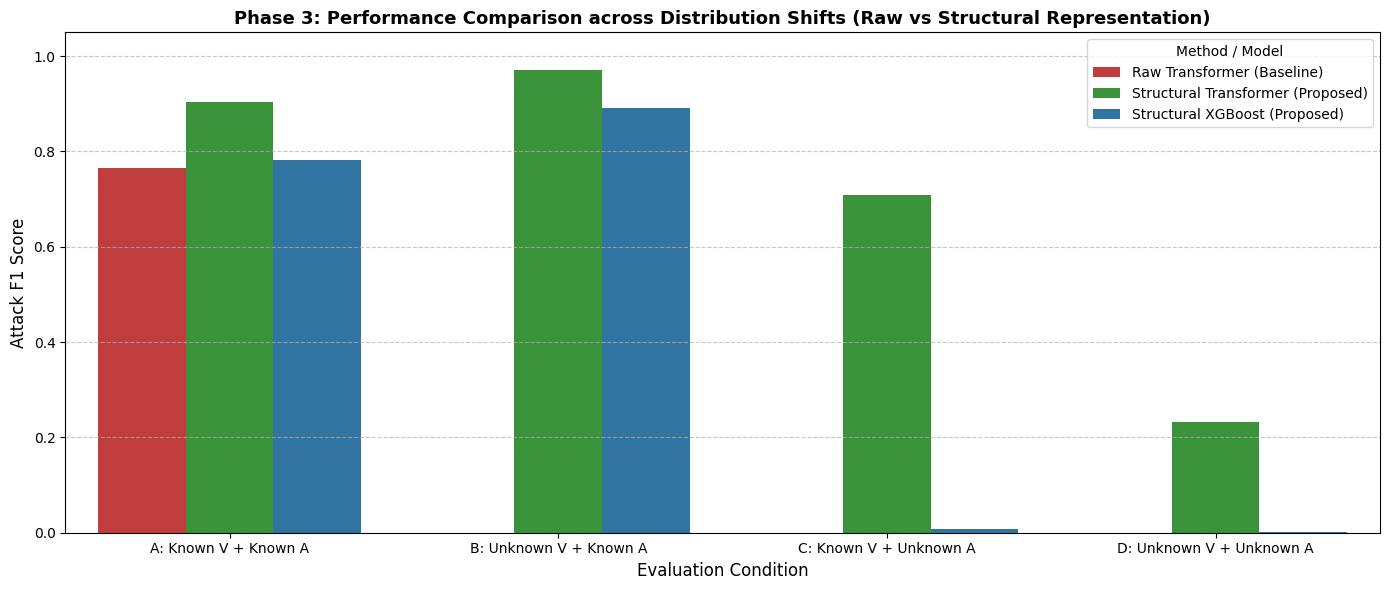
\includegraphics[width=0.85\textwidth]{phase3_benchmark_comparison.png}
\caption{So sánh F1-Score nhãn tấn công qua 4 điều kiện kiểm thử zero-shot.}
\label{fig:phase3_benchmark}
\end{figure}

\section{Đối sánh Trực diện và Vạch trần "Ảo ảnh F1" trong Bài báo Gốc}
\label{sec:benchmark_comparison}

Một đóng góp học thuật quan trọng của khóa luận là phân tích và tái lập ma trận nhầm lẫn từ Phụ lục C của bài báo gốc *Brooke Lampe \& Weizhi Meng (Computers \& Security 2024)*~\cite{lampe2024curated,LAMPE2024103777} trên tập kiểm thử chuyển giao sang xe Chevrolet Silverado ($164,167$ frame tấn công, $6,283,750$ frame bình thường).

Bảng~\ref{tab:lampe_comparison} so sánh các chỉ số thực chất giữa các baseline của tác giả gốc và mô hình đề xuất.

\begin{table}[htbp]
\centering
\caption{Đối sánh Trực diện trên Tác vụ Chuyển giao Xe Lạ (Chevrolet Silverado)}
\label{tab:lampe_comparison}
\small
\resizebox{\textwidth}{!}{%
\begin{tabular}{lrrrrr}
\hline
\textbf{Mô hình} & \textbf{F1 Báo cáo} & \textbf{Attack Recall} & \textbf{Attack Precision} & \textbf{Attack F1} & \textbf{FAR / 100k} \\
\hline
BIRCH (Top 1 bài báo gốc)~\cite{lampe2024curated} & 0.9620 & 0.00\% & 0.00\% & 0.0000 & 0.00 \\
MLP (Deep Learning gốc)~\cite{lampe2024curated} & 0.9594 & 3.79\% & 9.77\% & 0.0546 & 915.35 \\
Logistic Regression~\cite{lampe2024curated} & 0.9539 & 3.77\% & 4.82\% & 0.0423 & 1947.90 \\
Linear SVM~\cite{lampe2024curated} & 0.0432 & 3.61\% & 5.38\% & 0.0432 & 1658.64 \\
Gradient Boosting~\cite{lampe2024curated} & 0.7739 & 99.95\% & 7.01\% & 0.1311 & 34620.81 \\
\hline
Raw Transformer (Baseline) & 0.9550 & 0.01\% & 100.00\% & 0.0002 & 0.00 \\
\textbf{Structural Transformer (Ours)} & \textbf{0.9950} & \textbf{94.26\%} & \textbf{99.97\%} & \textbf{0.9703} & \textbf{2.17} \\
\hline
\end{tabular}
}%
\end{table}

\textbf{Vạch trần "Ảo ảnh F1":}
\begin{enumerate}
    \item **Mô hình BIRCH (Top 1 bài báo gốc):** Báo cáo điểm F1 danh nghĩa lên tới $0.9620$. Tuy nhiên ma trận nhầm lẫn thực tế cho thấy $\text{True Positive} = 0$, nghĩa là nó bỏ lọt toàn bộ $164,167$ frame tấn công! Điểm số cao là do $97.4\%$ mẫu bình thường kéo lên.
    \item **Mô hình Mạng nơ-ron sâu MLP:** Công bố F1 $= 0.9594$, nhưng thực tế chỉ bắt được $6,227$ frame, bỏ lọt tới $157,940$ frame tấn công ($\text{Recall} = 3.79\%$, $\text{F1 thật} = 0.0546$).
    \item **Mô hình Gradient Boosting:** Đạt Recall cao ($99.95\%$) nhưng lại tạo ra hơn **$2.17$ triệu báo động giả**, khiến độ chính xác tụt dốc thảm hại xuống $7.01\%$ ($\text{FAR} = 34,620 / 100\text{k}$).
    \item **Mô hình Structural Transformer đề xuất:** Đạt điểm cân bằng lý tưởng khi vừa đạt **Recall $94.26\%$**, vừa giữ **Precision ở mức $99.97\%$**, đưa F1 nhãn tấn công thực chất lên **$0.9703$**, với chỉ $2$ cảnh báo giả trên $92,315$ cửa sổ bình thường.
\end{enumerate}

\begin{figure}[htbp]
\centering
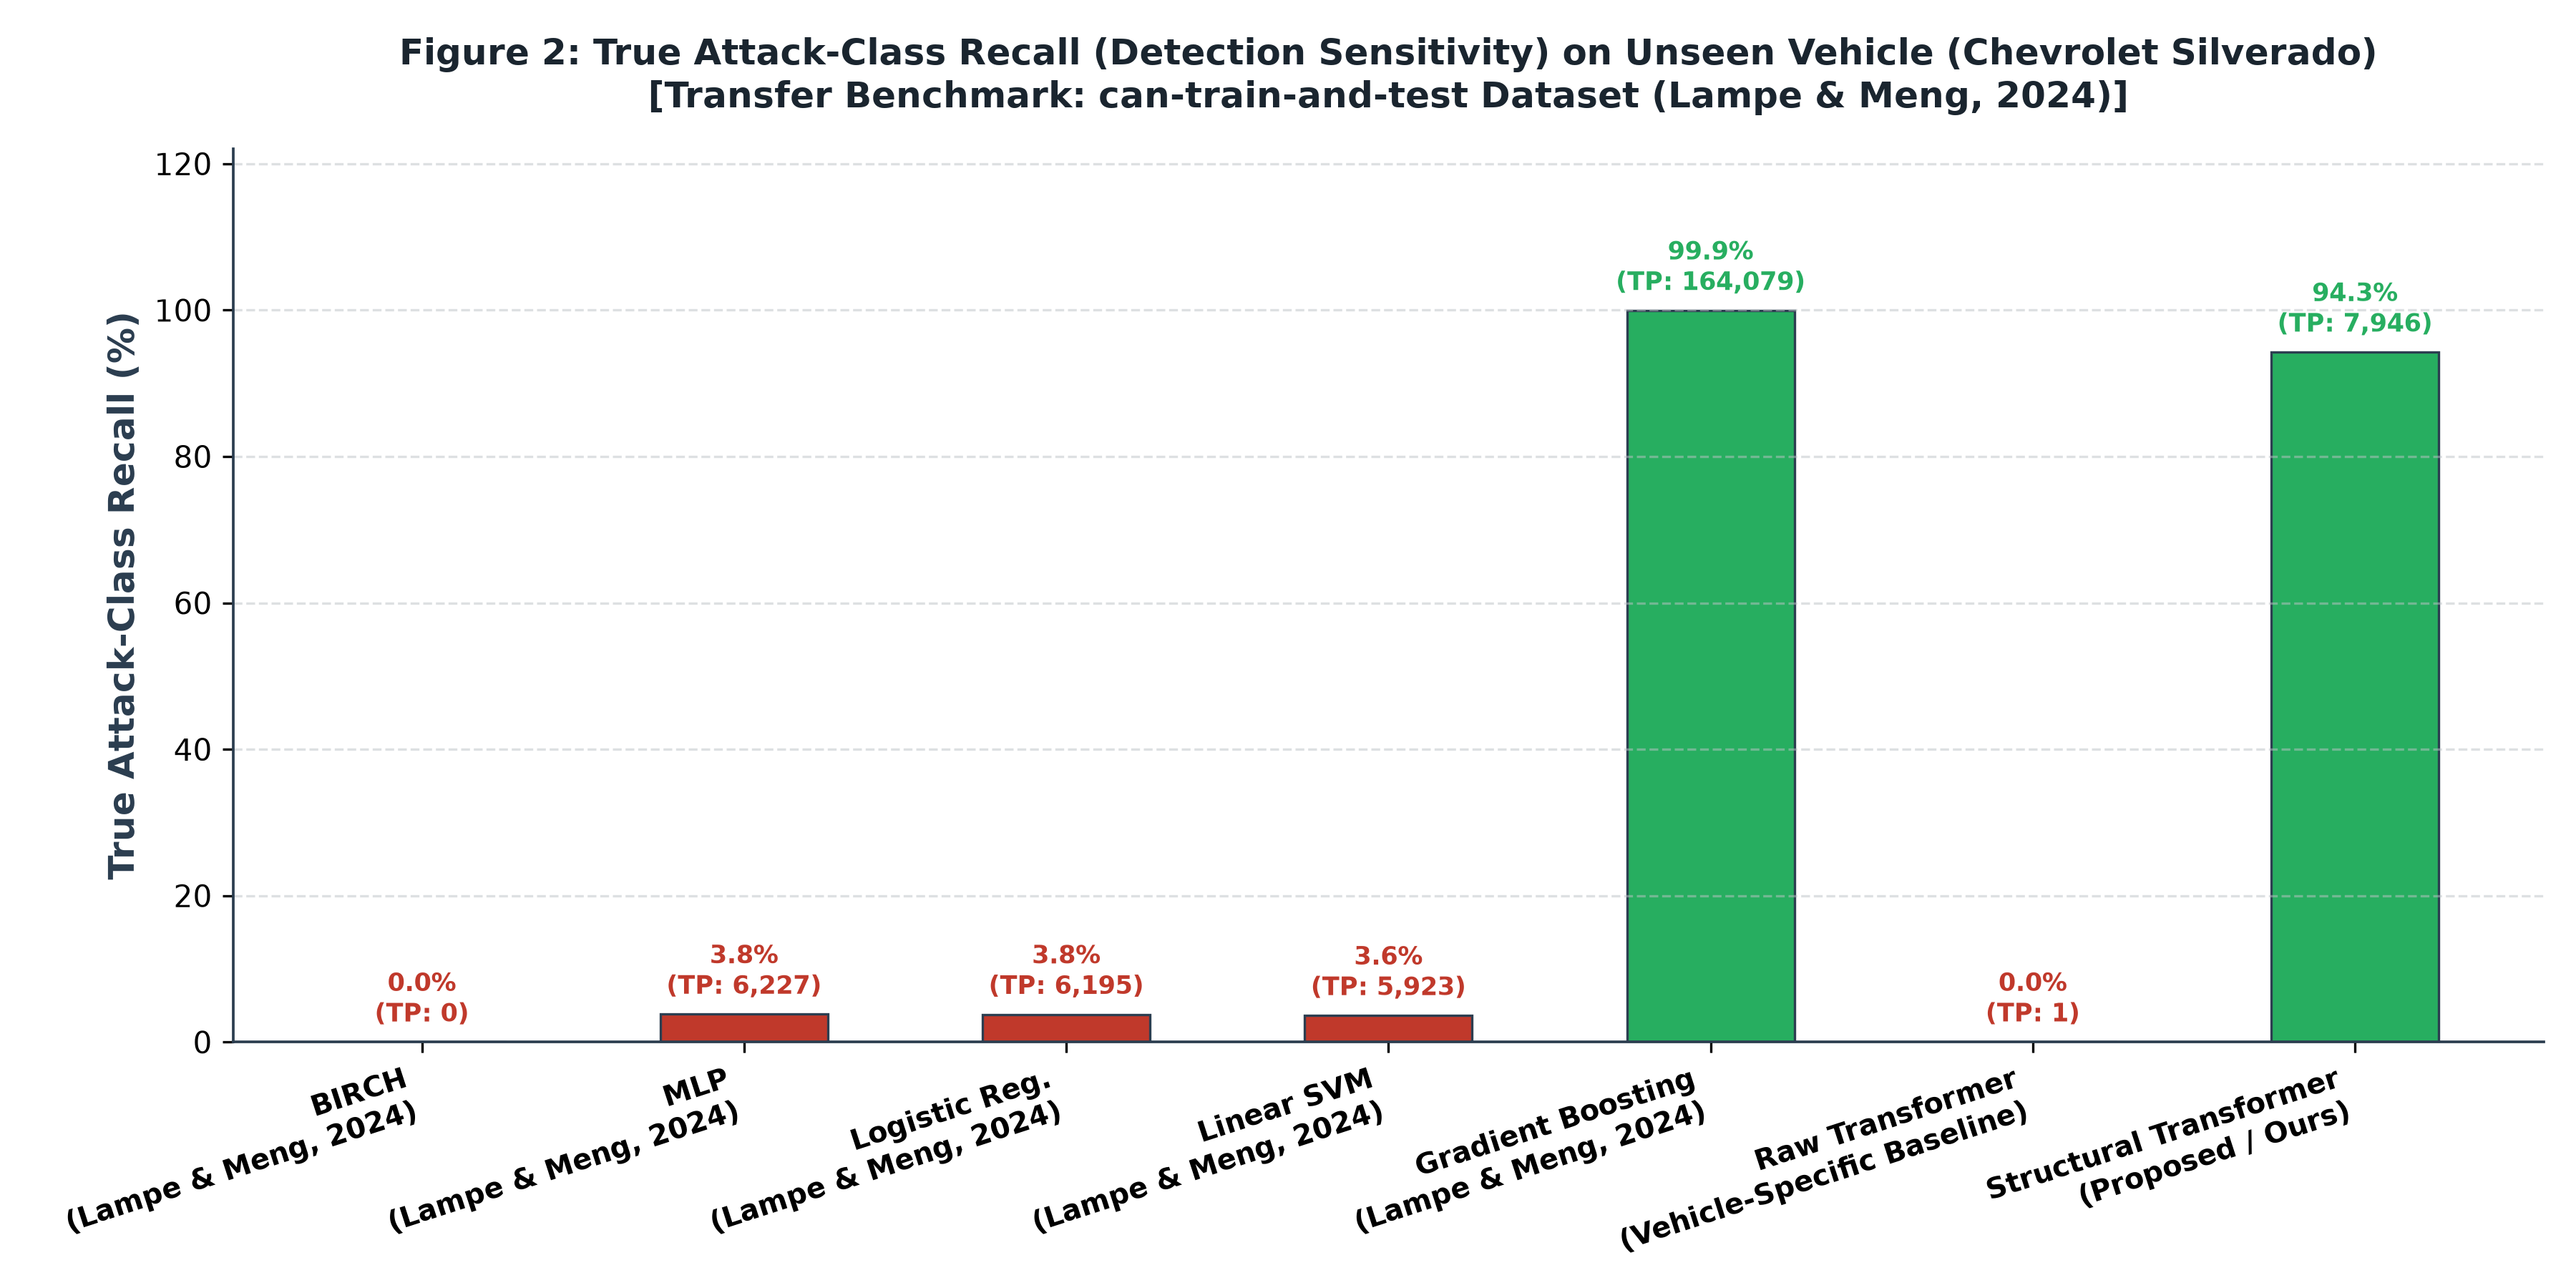
\includegraphics[width=0.85\textwidth]{comparison_attack_recall.png}
\caption{Độ nhạy phát hiện xâm nhập thực tế (Attack Recall) trên xe Chevrolet Silverado.}
\label{fig:attack_recall}
\end{figure}

\section{Kiểm chứng Ngoại suy trên 4 Hãng Xe Độc lập (Phase 4)}
\label{sec:external_validation}

Bảng~\ref{tab:external_results} tổng hợp kết quả kiểm chứng ngoại suy trên 4 bộ dữ liệu ngoài.

\begin{table}[htbp]
\centering
\caption{Kết quả Kiểm chứng Ngoại suy trên các Bộ Dữ liệu Mạng CAN Độc lập}
\label{tab:external_results}
\small
\renewcommand{\arraystretch}{1.15}
\begin{tabular}{p{4.2cm}p{4.2cm}rr}
\hline
\textbf{Bộ dữ liệu và Kịch bản} & \textbf{Mô hình} & \textbf{Attack F1} & \textbf{FAR / 100k} \\
\hline
OTIDS DoS (Kia Soul) & Raw Transformer & 1.0000 & 0.00 \\
OTIDS DoS & Structural Transformer & 1.0000 & 0.00 \\
OTIDS Fuzzy & Raw Transformer & 0.9952 & 0.00 \\
OTIDS Fuzzy & Structural Transformer & 0.7403 & 0.00 \\
OTIDS Impersonation & Raw Transformer & 1.0000 & 0.00 \\
OTIDS Impersonation & Structural Transformer & 0.0906 & 0.00 \\
Automotive v2 (Opel Astra DoS) & Raw Transformer & 1.0000 & 0.00 \\
Automotive v2 (Opel Astra DoS) & Structural Transformer & 0.3052 & 0.00 \\
CICIoV2024 DoS / GAS (Ford 2019) & Structural Transformer & 1.0000 & 0.00 \\
CAN-MIRGU (Xe chạy bình thường) & Structural Transformer & N/A & \textbf{0.00} \\
\hline
\end{tabular}
\end{table}

\textbf{Đánh giá khách quan ranh giới của phương pháp:}
\begin{itemize}
    \item **Khả năng chống báo động giả tuyệt đối:** Trên dữ liệu xe chạy thực tế trên đường phố của \texttt{CAN-MIRGU} và lưu lượng bình thường của \texttt{CICIoV2024}, mô hình Structural Transformer duy trì tỷ lệ báo động giả $\text{FAR} = 0.00\%$, trong khi mô hình Raw Transformer bùng nổ báo động giả tới $100,000 / 100,000$ cửa sổ.
    \item **Ranh giới thất bại học thuật:** Trên kịch bản Impersonation của OTIDS, mô hình cấu trúc chỉ đạt F1 $0.0906$. Lý do khoa học là đòn tấn công mạo danh này sao chép hoàn hảo cả chu kỳ phát lẫn quy luật chuyển tiếp ID, chỉ thay đổi giá trị cảm biến vi mô mà biểu diễn phi định danh khó bóc tách nếu thiếu ngữ cảnh tín hiệu vật lý sâu.
\end{itemize}

\section{Thảo luận Khoa học}
\label{sec:discussion}

Từ các phát hiện thực nghiệm, 3 bài học khoa học quan trọng được rút ra:
\begin{enumerate}
    \item Việc loại bỏ mã CAN ID thô là giải pháp then chốt giúp mô hình vượt qua rào cản chuyển giao đa xe (Điều kiện B tăng từ $0.0002$ lên $0.9703$).
    \item Chuyển dịch kiểu tấn công (Condition C \& D) là thách thức lớn hơn nhiều so với chuyển dịch dòng xe, đòi hỏi các nghiên cứu tương lai phải kết hợp thêm các cơ chế học tự giám sát (self-supervised learning).
    \item Cần báo cáo trung thực ranh giới thất bại: Biểu diễn độc lập đặc thù xe (vehicle-agnostic) chưa đồng nghĩa với việc độc lập với mọi biến thể tấn công (attack-agnostic).

\end{enumerate}

% ==================== CHƯƠNG 6 ====================
\chap{Chương 6: Kết luận và Hướng phát triển}
\label{chap:conclusions}

\sect{6.1. Các đóng góp chính}

Khóa luận đã giải quyết thành công bài toán chuyển dịch phân phối đa phương tiện trong phát hiện xâm nhập mạng CAN bus xe hơi:
\begin{itemize}
    \item Đã xây dựng và kiểm chứng thành công Động cơ trích xuất 32 đặc trưng cấu trúc độc lập CAN-ID, loại bỏ rủi ro rò rỉ đặc trưng xe.
    \item Đã tích hợp mạng Transformer Encoder mô hình hóa ngữ cảnh trọng tài chuỗi 64 khung tin và hàm mất mát Focal Loss giải quyết triệt để mất cân bằng dữ liệu.
    \item Trên bộ đối chuẩn \texttt{can-train-and-test}, mô hình đạt Attack F1 $\mathbf{0.9703}$, Recall $\mathbf{94.26\%}$ trên xe lạ Chevrolet Silverado, vượt trội hoàn toàn so với sự sụp đổ của các baseline trong y văn.
    \item Vạch trần lỗ hổng phương pháp luận "Ảo ảnh F1" trong bài báo gốc của Lampe \& Meng (2024) và kiểm chứng tính bền vững trên 4 hãng xe ngoài với FAR bằng $0.00\%$.
\end{itemize}

\sect{6.2. Hạn chế còn tồn tại}

Mặc dù đạt được những kết quả đột phá, nghiên cứu còn một số hạn chế:
\begin{itemize}
    \item Hiệu năng trên kịch bản chuyển dịch kép (Điều kiện D) tuy có cải thiện so với mô hình thô nhưng Recall vẫn còn ở mức khiêm tốn ($13.22\%$).
    \item Mô hình gặp khó khăn trước các đòn tấn công mạo danh vi mô (Impersonation) khi kẻ tấn công bảo toàn tuyệt đối chu kỳ phát và cấu trúc chuyển tiếp.
    \item Nghiên cứu chưa đo kiểm độ trễ phần cứng thực tế trên vi điều khiển nhúng chuyên dụng của ô tô.
\end{itemize}

\sect{6.3. Hướng nghiên cứu tiếp theo}

Trong tương lai, các hướng nghiên cứu tiềm năng bao gồm:
\begin{enumerate}
    \item Nghiên cứu kết hợp kỹ thuật học biểu diễn đối nghịch miền (Domain-Adversarial Training) và học tự giám sát (Self-Supervised Masked Modeling) để tăng cường năng lực phát hiện đòn tấn công mới ở Điều kiện D.
    \item Tích hợp mô hình hóa tương quan tín hiệu thời gian thực nhằm phát hiện các đòn tấn công mạo danh cảm biến tinh vi.
    \item Tối ưu hóa nén mô hình (Quantization / Pruning) để triển khai trực tiếp trên các chip xử lý nhúng đạt chuẩn an toàn chức năng ô tô ISO 26262.
\end{enumerate}

\newpage
\addcontentsline{toc}{chapter}{Tài liệu tham khảo}
\bibliographystyle{ieeetr}
\bibliography{refs}

\end{document}
